%%
%% Berliner Hochschule für Technik --  Projektarbeit/Projekt-Labor
%%
%% Chapter 1
%%
%%

%TODO After release of this document: 
%1) adjust to code style
%2) make a release with changelog


\chapter{Introduction}
\label{chap:Introduction}

The scope of the project is to produce an algorithm for the solar charge controller (mppt-1210-hus) \footnote{\url{https://github.com/LibreSolar/mppt-1210-hus}} produced by libre.solar, which outputs the state of charge (SoC) of the lead acid battery attached to it.

%TODO put a schematic of photo of the setup here, could be the design of the controller as well.

A key principle followed throughout the project is to use, wherever possible, Free Open-source Hardware (FOSH) and Free Open-source Software (FOSS). Consequently, the whole project has been
released as source code with a license adhering to these principles \cite{Schons_Development_and_validation_2021} is available at \footnote{ \url{https://github.com/mulles/Doc_Projekt-Labor_SOC} }. As the SoC can only be measured indirectly, it has to be deduced from available measurements.  %TODO at citations here that prove this
The charge controller exposes battery current and voltage measurements once a second for this purpose. \\%TODO make a table out of this list or some other structure with label which can be referenced in implementations
There are three main approaches for estimating the SoC: model-based, data-driven, coulomb-counting w/ Open circuit voltage (OCV) \cite{espedal2021current}. Best results seems to be achieved with combining the approaches to profit from their different strengths.

%\section{Background}

\subsubsection{Current integration method - Coulomb Counting /w OCV }
\label{section:CoulombCounting}

Seems the most simple way to define SoC:

\begin{equation}
z(t) = z(0) - \frac{1}{{Q_{C}}}\int_{0}^{\Delta t} {i(t)\ dt}
\label{equations:CoulombCounting}
\end{equation}
where: 
\begin{tabbing}
\phantom{$v(t)  \  \ \ \ $}\= \kill
$z  $\> = the SoC  \\
$i  $\> = battery current  \\
$Q_{C}$\> =  battery capacity   \\
$\Delta t$\> = the time interval between two current measurements
\end{tabbing}

The initial SoC $z(0)$ is determined by consulting a OCV-SoC lookup table. Starting from there the charge in relation to total capacity entering and leaving the battery is subtracted from SoC. This method has several disadvantages: \\
%TODO make a table out of this list or some other structure with label which can be referenced
-The initial SoC incorporates already an error, which won't be corrected till recalibration \\
-Error in counting charges and measurement errors accumulate quickly\\
-The algorithms only recalibrate reliably on full charge, which especially in solar systems does not occur regularly, producing awful SoC till recalibration. \\ %TODO at citations here that prove this

The coulomb counting method is most often combined with ongoing voltage measurements, while battery is at rest, known as OCV and a resulting OCV-SoC-lookup as shown in figure \ref{fig:OCVLead}. This mitigates the recalibration problem in case the battery gets some rests, but this enhancement still does not take hysteresis into account, which make OCV-SoC-lookup even with voltages at rest unreliable \cite{6861809} \cite{khan2016hysteresis}. %OCV-SoC curve is very flat for mid range SoC for LiPo.


%\hyperlink{datasheetBattery}{Datasheet Lead acid battery}

\begin{pylabcode}[plotsession]
rc('text', usetex=True)
rc('font', **{'family':'serif', 'serif':['Times']})
rc('font', size=10.0)			
rc('legend', fontsize=10.0)

# Kalman-Soc original Data embedded in kalman-soc/src/SoCKalman.cpp , quality seems at least possible. See of # the battery we are using: 
# https://eu.industrial.panasonic.com/sites/default/pidseu/files/downloads/files/id_vrla_handbook_e.pdf

xDataLead = [ 0, 1000, 2000, 3000, 4000, 5000, 6000, 7000, 8000, 9000, 10000, 11000, 12000, 13000, 14000, 15000, 16000, 17000, 18000, 19000, 20000, 21000, 22000, 23000, 24000, 25000, 26000, 27000, 28000, 29000, 30000, 31000, 32000, 33000, 34000, 35000, 36000, 37000, 38000, 39000, 40000, 41000, 42000, 43000, 44000, 45000, 46000, 47000, 48000, 49000, 50000, 51000, 52000, 53000, 54000, 55000, 56000, 57000, 58000, 59000, 60000, 61000, 62000, 63000, 64000, 65000, 66000, 67000, 68000, 69000, 70000, 71000, 72000, 73000, 74000, 75000, 76000, 77000, 78000, 79000, 80000, 81000, 82000, 83000, 84000, 85000, 86000, 87000, 88000, 89000, 90000, 91000, 92000, 93000, 94000, 95000, 96000, 97000, 98000, 99000, 100000 ]
yDataLead = [ 11640, 11653, 11666, 11679, 11692, 11706, 11719, 11732, 11745, 11758, 11772, 11785, 11798, 11811, 11824, 11838, 11851, 11864, 11877, 11890, 11904, 11917, 11930, 11943, 11956, 11970, 11983, 11996, 12009, 12022, 12036, 12049, 12062, 12075, 12088, 12102, 12115, 12128, 12141, 12154, 12168, 12181, 12194, 12207, 12220, 12234, 12247, 12260, 12273, 12286, 12300, 12313, 12326, 12339, 12352, 12366, 12379, 12392, 12405, 12418, 12432, 12445, 12458, 12471, 12484, 12498, 12511, 12524, 12537, 12550, 12564, 12577, 12590, 12603, 12616, 12630, 12643, 12656, 12669, 12682, 12696, 12709, 12722, 12735, 12748, 12762, 12775, 12788, 12801, 12814, 12828, 12841, 12854, 12867, 12880, 12894, 12907, 12920, 12933, 12946, 12960 ]
xLead = []
yLead = []
for OCV in xDataLead:
    xLead.append(OCV / 1000)
for SoC in yDataLead:
    yLead.append(SoC / 1000)

# Kalman-Soc original Data embedded in  
# kalman-soc/src/SoCKalman.cpp , something seems wrong with this data as it goes from 5V to 12.960   

xDataLi = [ 0, 1000, 2000, 3000, 4000, 5000, 6000, 7000, 8000, 9000, 10000, 11000, 12000, 13000, 14000, 15000, 16000, 17000, 18000, 19000, 20000, 21000, 22000, 23000, 24000, 25000, 26000, 27000, 28000, 29000, 30000, 31000, 32000, 33000, 34000, 35000, 36000, 37000, 38000, 39000, 40000, 41000, 42000, 43000, 44000, 45000, 46000, 47000, 48000, 49000, 50000, 51000, 52000, 53000, 54000, 55000, 56000, 57000, 58000, 59000, 60000, 61000, 62000, 63000, 64000, 65000, 66000, 67000, 68000, 69000, 70000, 71000, 72000, 73000, 74000, 75000, 76000, 77000, 78000, 79000, 80000, 81000, 82000, 83000, 84000, 85000, 86000, 87000, 88000, 89000, 90000, 91000, 92000, 93000, 94000, 95000, 96000, 97000, 98000, 99000, 100000 ]
yDataLi = [ 5000, 6266, 7434, 8085, 8531, 8867, 9134, 9355, 9543, 9705, 9847, 9974, 10088, 10191, 10285, 10372, 10451, 10525, 10595, 10659, 10720, 10777, 10831, 10882, 10931, 10977, 11021, 11063, 11104, 11142, 11180, 11216, 11251, 11284, 11317, 11349, 11379, 11409, 11438, 11467, 11495, 11522, 11548, 11574, 11600, 11625, 11650, 11675, 11699, 11723, 11746, 11769, 11793, 11815, 11838, 11861, 11883, 11906, 11928, 11950, 11972, 11994, 12017, 12039, 12061, 12083, 12105, 12127, 12150, 12172, 12195, 12217, 12240, 12263, 12286, 12309, 12333, 12356, 12380, 12404, 12428, 12452, 12477, 12501, 12526, 12552, 12577, 12603, 12629, 12655, 12682, 12708, 12735, 12763, 12790, 12818, 12846, 12875, 12903, 12931, 12960 ]
xLi = []
yLi = []
for OCV in xDataLi:
    xLi.append(OCV / 1000)
for SoC in yDataLi:
    yLi.append(SoC / 1000)
    
    
#source:  https://web.calce.umd.edu/batteries/data.htm -> K2_016/6_27_13_1C_Charge.xlsx   LiFePO4 Battery K2 2600mAh
xLiPo =  [ 0,0,0.833490809379538,1.66722670558431,2.50096620570669,3.33427225436727,4.16801618996658,5.00133685566704,5.83550118428331,6.66879419861738,7.50297439411519,8.33673100316758,9.17005785722104,10.0042486341523,10.8380070163062,11.671765136375,12.505090758318,13.3392869176225,14.1730443196998,15.0063730151,15.8405714313937,16.6743304149022,17.5080879275519,18.3362054647438,19.1756146417219,20.008941095832,20.8427009935568,21.6764648915728,22.5097947538067,23.3439933490688,24.1773205700798,25.0115155212229,25.845273599529,26.6790441464923,27.5123634060736,28.3465621233068,29.1798886839182,30.0140868131342,30.8474159236465,31.6746712769722,32.5153784118575,33.348705551299,34.1824688853269,35.0162233363333,35.849995065367,36.6833233833931,37.5170891215189,38.3508443545727,39.1846133862124,40.018376674183,40.8521279110113,41.6854643407802,42.5192361189747,43.3529921363778,44.1867637666053,45.0205139900149,45.8542830285854,46.687613226699,47.5218127700638,48.3555786962652,49.1893364477339,50.0230989787774,50.8568645334109,51.6901927834099,52.5243936546185,53.3577223463532,54.1919158289088,55.0252423110576,55.859420072829,56.6927662322223,57.5260953659525,58.360298403603,59.1936255576868,60.0273946374812,60.8611621947514,61.6944942107511,62.5282541184676,63.3620208723698,64.1953496834188,65.029546606631,65.8628779572076,66.697075646007,67.5304012969913,68.3645922311219,69.1979204587838,70.0321202957886,70.8658796433478,71.6992082438051,72.5329663761915,73.3667342207558,74.2004810516524,75.0338169144245,75.867142415826,76.7008950667888,77.5346531938478,78.3684053179512,79.2021588865777,80.0359181938605,80.869667002119,81.7029838812077,82.5371651994041,83.3704815760764,84.204229285592,85.0379754632156,85.87172817679,86.7054748883744,87.3265586747438,87.9984653028184,88.4861917627595,88.8575394315189,89.1510852601711,89.3910142777207,89.5941295173262,89.7701928104088,89.9260092188262,90.0661973653891,90.1939858780953,90.3118160272713,90.4212251900254,90.5236183846095,90.6198018529033,90.7106851820891,90.7971558362801,90.8797961289026,90.9589946525035,91.0350007967055,91.1082101888731,91.1790805694922,91.2477155031653,91.3140685941997,91.3787347517039,91.441660047231,91.5027337175027,91.5623129774125,91.6206670224798,91.6777193524635,91.7334853253027,91.787995794269,91.84131183554,91.8936717439273,91.9451642015128,91.9957269838529,92.0454653256594,92.0944112072043,92.1426623900379,92.1897822430998,92.2370223930395,92.2830756656371,92.3283667671187,92.373024426061,92.4169771207322,92.4603327589931,92.5030950820185,92.5454478461459,92.5872829115937,92.6286319790374,92.6694675937403,92.7097933233886,92.7497554754121,92.7894706961655,92.8289291746393,92.8680346083796,92.9068555312024,92.9453915722361,92.9836157053954,93.021648998296,93.0592943658371,93.0965510721531,93.133319398869,93.1698747564757,93.2061945858012,93.2421388978153,93.2778711554555,93.3134225635469,93.3485085502716,93.3834482440598,93.4181219558929,93.4525693798099,93.4867144085467,93.5205374184425,93.554137460936,93.5875292208488,93.6206464452502,93.6535729966917,93.6863633858535,93.7188041302675,93.7510369715929,93.7831103138006,93.8150542869873,93.8468161212691,93.878287443082,93.9094877117766,93.9405302503893,93.9712600488479,94.0018844380903,94.0325311631932,94.0630841555871,94.0934808352906,94.1237558660206,94.153830507164,94.1838325694906,94.2136919163822,94.2432944108117,94.2728609260898,94.302324343062,94.3316929313469,94.3610321096233,94.3901685920118,94.4190456838146,94.4477653529343,94.4762210516353,94.5045029995084,94.532537828582,94.5604881336057,94.5883576006919,94.616081704923,94.6437769769233,94.671243173028,94.6986775157053,94.7260035940201,94.753212532215,94.7803330752399,94.8073439239682,94.834121803401,94.8607949845459,94.8874825572235,94.914219533141,94.9408932544463,94.9674630156808,94.9938712789982,95.0202731833489,95.046695257072,95.0729485198319,95.0990731199742,95.1250792266783,95.1510194226728,95.1768569061185,95.2027643212758,95.2284709868596,95.2540527038175,95.279694634934,95.305285253846,95.3309081937116,95.3564278874749,95.3817667959063,95.4069286351198,95.4320477119096,95.4569999761046,95.4820073905805,95.5069971994278,95.53190111773,95.5566078013798,95.5812054290854,95.6057295203875,95.6303516718585,95.6550421936167,95.679644778752,95.7042392517681,95.728842978987,95.7533932070913,95.777942216257,95.8024316539401,95.8268888314295,95.8512907190292,95.8756729198126,95.8999450039417,95.9241566476536,95.9482181843843,95.9721035691664,95.996082155484,96.0198535600344,96.0437891357898,96.0676483267341,96.0913490888865,96.1151771944253,96.1390062987932,96.1628238359977,96.1866716179361,96.2106111107018,96.2344528668216,96.2582703348183,96.2821270878271,96.305805617727,96.3293188557615,96.3526859105505,96.376080923274,96.3992992637845,96.422435359167,96.4455318646497,96.4685468106844,96.4916395763572,96.5146409447999,96.5377156983757,96.5607019169126,96.5835534631265,96.606122356499,96.6291746793828,96.6520042305223,96.674646311839,96.697173033512,96.7196484755661,96.742088365469,96.764454485946,96.7868155920854,96.8091343930861,96.8315824784471,96.8539448365704,96.8761653034179,96.8983012199131,96.9204387185295,96.9423769502946,96.9640777384462,96.9857110855885,97.0073252233478,97.0288072970281,97.0503146399637,97.0716495633155,97.0930524324215,97.1143547284254,97.1355861835631,97.156725188409,97.1778175212228,97.1988956204657,97.2199392428807,97.2407863393051,97.261565386003,97.282265338296,97.3029068013984,97.323403635258,97.3438661497963,97.364261049301,97.3847002738579,97.4050021398832,97.4252780770448,97.445393109866,97.4654427713119,97.4854513562429,97.5053518267192,97.5252202132154,97.5451389448128,97.5650773145466,97.5849977575504,97.6048590013842,97.6247136754531,97.6445637093388,97.6643285138519,97.6840999031425,97.7040373810812,97.7239086766096,97.7436978570604,97.7632896084255,97.7827947688084,97.802036968086,97.8213624069483,97.8405383524952,97.8597805333716,97.8789494773002,97.8981185326867,97.9172047030935,97.9362547747662,97.9552389803456,97.9742221485085,97.9931482231457,98.0120856798146,98.0308984744274,98.0495989040375,98.06833043215,98.0870766456613,98.1057886843259,98.1244732586894,98.1431615949192,98.1618070505278,98.1802939101308,98.1987399062177,98.2171637100591,98.2354968118162,98.2537854029281,98.2721633972802,98.2904933476046,98.3088630754363,98.3270221136032,98.3451470188059,98.3633691622321,98.3814308436553,98.3996033019406,98.4176932230334,98.4357435124071,98.4537356138305,98.471810291084,98.4898541184256,98.5078933756623,98.5259220065314,98.5439123319154,98.5619114832062,98.5798391008765,98.5976530633345,98.6154180624168,98.6331478509977,98.6508430649962,98.6685758463251,98.6862754482659,98.7039159221583,98.7215371985115,98.7391118621132,98.7566770533085,98.7742205063163,98.7917707189076,98.8093239051738,98.8267977621177,98.8442642735062,98.8616949305746,98.8791336700836,98.8965410900052,98.9139236722623,98.9312194672205,98.9484134778555,98.9656519885332,98.9829146245352,99.0002351732367,99.0174150587146,99.034611361109,99.0517602456818,99.068838684221,99.0859975449108,99.1031466510441,99.1202994043316,99.1373479220814,99.1544355697643,99.1714590632297,99.1884709357383,99.205459867448,99.2223926905118,99.2393795548117,99.2563864021641,99.273352909429,99.2902728194072,99.307219865193,99.3240142912413,99.3407637547441,99.3575192661582,99.3742928028446,99.391011023451,99.4076633971313,99.4243930328224,99.4410567703226,99.4576927639098,99.4742803943221,99.4909019027676,99.5074712729813,99.5240307376294,99.5406028431904,99.5571587662747,99.5736159267511,99.5900008653058,99.6063820961919,99.6226814702013,99.6383043431653,99.6383043431653,99.6383043431653 ]
yLiPo = [ 9.52044153213501,9.51558351516724,9.99021148681641,10.035391330719,10.0523943901062,10.0621104240417,10.0703687667847,10.0776557922363,10.0864005088806,10.0956308841705,10.1043748855591,10.1145765781403,10.1247789859772,10.1344950199127,10.1442110538483,10.1534407138824,10.1621854305267,10.170930147171,10.1801598072052,10.1884188652039,10.1966772079468,10.2039642333984,10.2122232913971,10.2185382843018,10.2253396511078,10.2311689853668,10.236513376236,10.2418570518494,10.2457430362701,10.2496297359467,10.2535164356232,10.2574024200439,10.2603170871735,10.2637181282043,10.2666327953339,10.2690618038178,10.2719764709473,10.2748911380768,10.277806520462,10.2797491550446,10.2831501960754,10.2855792045593,10.2884938716888,10.2909228801727,10.2948095798492,10.2972385883331,10.3006389141083,10.3040392398834,10.3074402809143,10.3098692893982,10.313755273819,10.3171563148499,10.3210422992706,10.3254146575928,10.3293013572693,10.3336737155914,10.3375597000122,10.34241771698,10.3467900753021,10.3511624336243,10.3565061092377,10.3613641262054,10.3662221431732,10.3715658187866,10.3769102096558,10.3817682266235,10.3875975608826,10.392941236496,10.3992569446564,10.405571937561,10.4114019870758,10.4177169799805,10.4240326881409,10.4318053722382,10.4386067390442,10.4458937644959,10.4541521072388,10.4628968238831,10.4716415405273,10.4808712005615,10.4910736083984,10.5017609596252,10.513420343399,10.5265367031097,10.5406250953674,10.5551991462708,10.572202205658,10.5906629562378,10.6110663414001,10.6334130764008,10.6596465110779,10.6873369216919,10.7189140319824,10.7538921833038,10.7942132949829,10.8384218215942,10.8899166584015,10.9482128620148,11.014767408371,11.093953371048,11.1862556934357,11.2970187664032,11.4310998916626,11.5962724685669,11.8046815395355,12.0665287971497,12.3001999855042,12.2992272377014,12.2987422943115,12.2992272377014,12.2992272377014,12.2992272377014,12.2992272377014,12.2992272377014,12.2992272377014,12.2992272377014,12.2992272377014,12.2997136116028,12.2987422943115,12.2992272377014,12.2992272377014,12.2997136116028,12.2992272377014,12.2997136116028,12.2992272377014,12.2992272377014,12.2992272377014,12.2987422943115,12.2992272377014,12.2992272377014,12.2987422943115,12.2992272377014,12.2992272377014,12.2992272377014,12.2992272377014,12.2987422943115,12.2987422943115,12.2987422943115,12.2987422943115,12.2987422943115,12.2987422943115,12.2987422943115,12.2992272377014,12.2992272377014,12.2992272377014,12.2992272377014,12.2992272377014,12.2987422943115,12.2987422943115,12.2992272377014,12.2987422943115,12.2992272377014,12.2987422943115,12.2992272377014,12.2982559204102,12.2987422943115,12.2992272377014,12.2992272377014,12.2987422943115,12.2987422943115,12.2987422943115,12.2992272377014,12.2987422943115,12.2992272377014,12.2992272377014,12.2992272377014,12.2987422943115,12.2992272377014,12.2987422943115,12.2987422943115,12.2987422943115,12.2992272377014,12.2992272377014,12.2992272377014,12.2987422943115,12.2987422943115,12.2987422943115,12.2992272377014,12.2987422943115,12.2992272377014,12.2987422943115,12.2987422943115,12.2987422943115,12.2987422943115,12.2987422943115,12.2987422943115,12.2987422943115,12.2992272377014,12.2992272377014,12.2992272377014,12.2992272377014,12.2987422943115,12.2992272377014,12.2987422943115,12.2992272377014,12.2992272377014,12.2987422943115,12.2992272377014,12.2987422943115,12.2997136116028,12.2992272377014,12.2987422943115,12.2992272377014,12.2992272377014,12.2992272377014,12.2992272377014,12.2992272377014,12.2992272377014,12.2992272377014,12.2987422943115,12.2987422943115,12.2987422943115,12.2992272377014,12.2987422943115,12.2982559204102,12.2992272377014,12.2992272377014,12.2997136116028,12.2987422943115,12.2987422943115,12.2987422943115,12.2987422943115,12.2987422943115,12.2987422943115,12.2987422943115,12.2987422943115,12.2997136116028,12.2992272377014,12.2987422943115,12.2982559204102,12.2992272377014,12.2987422943115,12.2987422943115,12.2992272377014,12.2987422943115,12.2992272377014,12.2992272377014,12.2992272377014,12.2992272377014,12.2982559204102,12.2992272377014,12.2987422943115,12.2987422943115,12.2992272377014,12.2987422943115,12.2992272377014,12.2987422943115,12.2987422943115,12.2997136116028,12.2992272377014,12.2992272377014,12.2992272377014,12.2992272377014,12.2992272377014,12.2987422943115,12.2997136116028,12.2987422943115,12.2987422943115,12.2992272377014,12.2987422943115,12.2987422943115,12.2987422943115,12.2987422943115,12.2992272377014,12.2992272377014,12.2987422943115,12.2992272377014,12.2987422943115,12.2987422943115,12.2992272377014,12.2992272377014,12.2987422943115,12.2987422943115,12.2987422943115,12.2992272377014,12.2987422943115,12.2987422943115,12.2987422943115,12.2987422943115,12.2992272377014,12.2982559204102,12.2987422943115,12.2992272377014,12.2987422943115,12.2992272377014,12.2987422943115,12.2987422943115,12.2982559204102,12.2992272377014,12.2987422943115,12.2987422943115,12.2992272377014,12.2992272377014,12.2992272377014,12.2992272377014,12.2992272377014,12.2992272377014,12.2992272377014,12.2997136116028,12.2987422943115,12.2987422943115,12.2987422943115,12.2987422943115,12.2987422943115,12.2987422943115,12.2987422943115,12.2992272377014,12.2992272377014,12.2992272377014,12.2992272377014,12.2992272377014,12.2992272377014,12.2987422943115,12.2987422943115,12.2987422943115,12.2992272377014,12.2992272377014,12.2987422943115,12.2992272377014,12.2992272377014,12.2992272377014,12.2982559204102,12.2987422943115,12.2982559204102,12.2987422943115,12.2992272377014,12.2992272377014,12.2992272377014,12.2992272377014,12.2987422943115,12.2992272377014,12.2987422943115,12.2987422943115,12.2987422943115,12.2992272377014,12.2987422943115,12.2987422943115,12.2992272377014,12.2987422943115,12.2987422943115,12.2987422943115,12.2987422943115,12.2987422943115,12.2992272377014,12.2987422943115,12.2987422943115,12.2992272377014,12.2992272377014,12.2987422943115,12.2987422943115,12.2992272377014,12.2987422943115,12.2987422943115,12.2992272377014,12.2992272377014,12.2987422943115,12.2987422943115,12.2987422943115,12.2987422943115,12.2987422943115,12.2982559204102,12.2992272377014,12.2987422943115,12.2992272377014,12.2992272377014,12.2987422943115,12.2987422943115,12.2987422943115,12.2987422943115,12.2992272377014,12.2987422943115,12.2987422943115,12.2987422943115,12.2987422943115,12.2987422943115,12.2992272377014,12.2987422943115,12.2992272377014,12.2987422943115,12.2987422943115,12.2987422943115,12.2987422943115,12.2992272377014,12.2987422943115,12.2987422943115,12.2987422943115,12.2987422943115,12.2987422943115,12.2992272377014,12.2987422943115,12.2987422943115,12.2987422943115,12.2992272377014,12.2982559204102,12.2987422943115,12.2987422943115,12.2987422943115,12.2987422943115,12.2987422943115,12.2987422943115,12.2992272377014,12.2997136116028,12.2992272377014,12.2992272377014,12.2987422943115,12.2987422943115,12.2992272377014,12.2992272377014,12.2987422943115,12.2982559204102,12.2987422943115,12.2992272377014,12.2992272377014,12.2987422943115,12.2992272377014,12.2992272377014,12.2987422943115,12.2987422943115,12.2987422943115,12.2987422943115,12.2992272377014,12.2987422943115,12.2992272377014,12.2987422943115,12.2992272377014,12.2987422943115,12.2987422943115,12.2987422943115,12.2992272377014,12.2987422943115,12.2987422943115,12.2987422943115,12.2987422943115,12.2992272377014,12.2992272377014,12.2987422943115,12.2992272377014,12.2992272377014,12.2987422943115,12.2987422943115,12.2992272377014,12.2987422943115,12.2987422943115,12.2987422943115,12.2992272377014,12.2987422943115,12.2992272377014,12.2987422943115,12.2987422943115,12.2992272377014,12.2992272377014,12.2987422943115,12.2987422943115,12.2992272377014,12.2987422943115,12.2992272377014,12.2982559204102,12.1214246749878,11.974226474762 ]
    
    

 
figure(figsize=(3.25,2))
plot(xLead,yLead)
xlabel(r'SoC(\%)')
ylabel(r'OCV(V)')
#plot(xLiPo,yLiPo)
savefig('OCVlead.pdf', bbox_inches='tight')
\end{pylabcode}

\begin{figure}
\centering
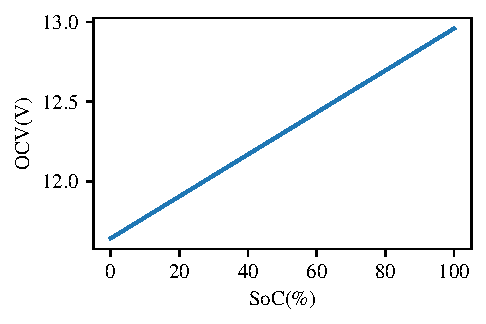
\includegraphics{OCVlead}
\caption{\label{fig:OCVLead} OCV-SoC lead acid battery }
\end{figure}


%\begin{pylabcode}[plotsession]
%rc('text', usetex=True)
%rc('font', **{'family':'serif', 'serif':['Times']})
%rc('font', size=10.0)			
%rc('legend', fontsize=10.0)
%
%
%#Kalman-Soc original Data embedded in  
%#kalman-soc/src/SoCKalman.cpp , something seems wrong with this data as it goes from 5V to 12.960V  
%xDataLi = [ 0, 1000, 2000, 3000, 4000, 5000, 6000, 7000, 8000, 9000, 10000, 11000, 12000, 13000, 14000, 15000, 16000, 17000, 18000, 19000, 20000, 21000, 22000, 23000, 24000, 25000, 26000, 27000, 28000, 29000, 30000, 31000, 32000, 33000, 34000, 35000, 36000, 37000, 38000, 39000, 40000, 41000, 42000, 43000, 44000, 45000, 46000, 47000, 48000, 49000, 50000, 51000, 52000, 53000, 54000, 55000, 56000, 57000, 58000, 59000, 60000, 61000, 62000, 63000, 64000, 65000, 66000, 67000, 68000, 69000, 70000, 71000, 72000, 73000, 74000, 75000, 76000, 77000, 78000, 79000, 80000, 81000, 82000, 83000, 84000, 85000, 86000, 87000, 88000, 89000, 90000, 91000, 92000, 93000, 94000, 95000, 96000, 97000, 98000, 99000, 100000 ]
%yDataLi = [ 5000, 6266, 7434, 8085, 8531, 8867, 9134, 9355, 9543, 9705, 9847, 9974, 10088, 10191, 10285, 10372, 10451, 10525, 10595, 10659, 10720, 10777, 10831, 10882, 10931, 10977, 11021, 11063, 11104, 11142, 11180, 11216, 11251, 11284, 11317, 11349, 11379, 11409, 11438, 11467, 11495, 11522, 11548, 11574, 11600, 11625, 11650, 11675, 11699, 11723, 11746, 11769, 11793, 11815, 11838, 11861, 11883, 11906, 11928, 11950, 11972, 11994, 12017, 12039, 12061, 12083, 12105, 12127, 12150, 12172, 12195, 12217, 12240, 12263, 12286, 12309, 12333, 12356, 12380, 12404, 12428, 12452, 12477, 12501, 12526, 12552, 12577, 12603, 12629, 12655, 12682, 12708, 12735, 12763, 12790, 12818, 12846, 12875, 12903, 12931, 12960 ]
%xLi = []
%yLi = []
%for OCV in xDataLi:
%    xLi.append(OCV / 1000)
%for SoC in yDataLi:
%    yLi.append(SoC / 1000)
%    
% 
%figure(figsize=(3.25,2))
%plot(xLi,yLi)
%xlabel(r'SoC(\%)')
%ylabel(r'OCV(V)')
%savefig('OCVLion.pdf', bbox_inches='tight')
%\end{pylabcode}

%\begin{figure}[!ht]
%\centering
%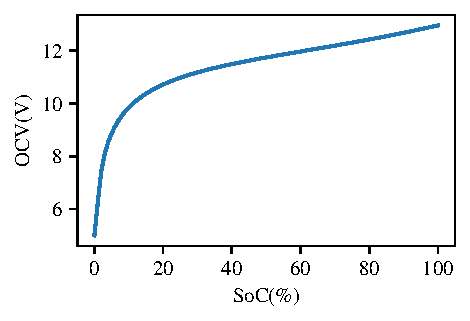
\includegraphics{OCVLion}
%\caption{\label{fig:OCVLion} OCV Lithium }
%\end{figure}


\pagebreak

The existing SoC function $Charger::update\_soc$  \footnote{\url{https://github.com/LibreSolar/charge-controller-firmware/blob/5196694e42c38eee18ab25e65bd51ec578eba101/src/bat_charger.cpp\#L325}} \ref{code:libreSolarSoC} embebbed in mppt-1210-hus uses OCV-SoC-lookup function based on linear interpolation of 
$ocv\_empty$ and $ocv\_full$:

%TODO reference code appendix




\begin{figure}
\centering
\includegraphics[width=15cm]{StateMaschineMartinLibreSolar3-s2.0-B9780444595133000157-f15-06ab-9780444595133.jpg}
\caption{\label{fig:StateMaschineMartinLibreSolar3} State maschine libre.solar}
\end{figure}
TODO Remove \ref{fig:StateMaschineMartinLibreSolar3}  and produce one that fits Libre.solar Algo maybe cite \url{https://www.sciencedirect.com/topics/engineering/coulomb-counting}  but it does not seems to be a good reference. 



\pagebreak

\subsubsection{Equivalent circuit based models}
\label{section:Equivalentcircuitbasedmodels}
\
\
\
\begin{figure}[h!]
\begin{center}

%\fbox{\includegraphics[
%    page=1,
%    width=15cm,
%    keepaspectratio,
%    trim=0.5cm 5.9cm 0.5cm 5cm
%]{ECMThevinModel} }


\includegraphics{g10} % [trim=0.5cm 5.9cm 0.5cm 5cm]
\caption{\label{fig:ECMThevinModel} Equivalent circuit model }
\end{center} 
\end{figure} 
 \\
The figure \ref{fig:ECMThevinModel} shows an empirical model known as Thévenin model or equivalent circuit model (ECM), adhering to the equation: 

\begin{equation}
{v}(t) = {OCV}(z(t))  - {R}_{0} i(t) - {R}_{1} {i}_{R_1}(t) 
\label{equation:ECM}
\end{equation}
where: 
\begin{tabbing}
\phantom{$v(t)  \  \ \ \ \ \ \ \ \ \ \ \ $}\= \kill
$v$\> =  voltage measured on battery terminals under load   \\
$z  $\> =  SoC  \\
$v_	1$\> =  ${R}_{1} {i}_{R_1}(t)$ \\
$OCV $\>  = a function based on a SoC-OCV-lookup table \\
$R_1,C_1,R_0$\> = don't exist as physical components inside the battery, their values are chosen to fit  \\
battery test data for example that of a hybrid pulse power characterization (HPPC) battery test  \\ % TODO  \cite{bibid} \url{http://mocha-java.uccs.edu/ECE5720/ECE5720-Notes02.pdf} page 2

\end{tabbing}

Other empirical models are the auto regressive exogenous (ARX) model and dual polarisation (DP) model. %TODO \cite{26. Xia, B.; Zheng, W.; Zhang, R.; Lao, Z.; Sun, Z. A Novel Observer for Lithium-Ion Battery State of Charge Estimation in Electric Vehicles Based on a Second-Order Equivalent Circuit Model. Energies 2017, 10, 1150. [CrossRef}.

\subsubsection{Physics based models}
\label{section:Physics based models}

As Gregory Plettv puts it in his lectures notes of course ECE5720  \footnote{ \url{http://mocha-java.uccs.edu/ECE5720/ECE5720-Notes02.pdf}} :  "Battery management and controls using physics-based models is a major focus of our present research efforts and (I hope) of a future
course" in 2015. The first papers on the topic are available now \cite{9477587}, but physics based models (PBM) still are hard to implement and not much material or software code is available. Thus, the ECM model is preferred for now. Moreover, the PBM based models have a higher computational complexity than
empirical models, making it non suitable for the mppt-1210-hus micro-controller unit (MCU) being a 32bit ARM STM32L072. %TODO find another citation of gregory plett concerning PBM's


\subsubsection{Data-driven}
\label{section:Data-driven}

These approaches are based on artificial

intelligence (AI) and need good training data and the right training parameters. Combined with PBM's it is a very promising research field \cite{9477587}, which first successes to reduce the computational complexity so online estimation of SoC on MCU is	 possible.


%\chapter{Hardware Setup for validation}

%\begin{figure}[!ht]
%\includegraphics{SOC_Setup.png}
%\caption{\label{fig:SoCSetup} Setup to verify SoC Algorithm}
%\end{figure}

%TODO this might just be ignored for now, as it would double the size of this document. It could be used so the user gets an idea of how the system looks like. Maybe a more simple schematic or photo incorpated in the introduction \ref{chap:Introduction}  would make more sense. The setup might not even have been used to produce data for this project, more to learn about the system the algo has been developed for.

\chapter{Implementation}
\label{chap:Implementation}

%3 steps for SoC Algo implementation: \\
%1) model design\\  2) identification of model parameters \\ 3) SoC determination \\

It is popular to combine %hybrid approach 
any of the approaches introduced in \ref{chap:Introduction} with a kalman filter (KF) in order to reduce the influence of white (uncorrelated) noise in measurements and to combine voltage and current measurements known as sensor fusion. The second principle makes the algorithm resilient to inaccurately chosen ECM parameters. In this project the combination of coulomb counting \ref{section:CoulombCounting} and ECM \ref{section:Equivalentcircuitbasedmodels} has been chosen. \\ %\cite{} a couple of papers making use of KF in combinations with different approaches see  As for battery states estimation, the Kalman filter family has been extensively used to estimate the SOC, e.g., the extended Kalman filter (EKF). of paper Online Parameters Identification and State of Charge Estimation for Lithium-Ion Battery Using Adaptive Cubature Kalman Filter
%TODO cite \url{https://okrasolar.com/blog/building-a-lightweight-state-of-charge-algorithm/}  
\\
As the  ECM's equation \ref{equation:ECM}  is non-linear an extended kalman filter (EKF) needs to be used. The EKF linearizes the non-linear system by calculating the Jacobian matrix, which is the Taylor series expansions of first order.  %\cite{Online Parameters Identification and State of Charge Estimation for Lithium-Ion Battery Using Adaptive Cubature Kalman Filter}. 
\\

\section{EFK implementation}
\label{Fork}

A reasonable step by step guide to implement the EKF is \cite{rzepka2021implementing}. The algorithm refined in this project is based on a fork of the algorithm named $kalman-soc$\footnote{ \url{https://github.com/mulles/kalman-soc}} designed by Matthew Johnston for the company okra-solar. 

The refinements consists of improvements or adaptions to libre.solar use case and code base.
\\


%TODO verify if this it completely wrong: -Works without the input of a Equivalent Circuit Model (ECM) specific to the physical battery, which would need to be parameterized doing advanced measurements during charging and discharging of the battery. 


%TODO make a table out of this list or some other structure with label which can be referenced
Changelog\footnote{note exact changes are traceable with the commits to the fork. 
}: 

\begin{itemize}
\item adoption of libre solar code style guide 

\item adoption of TinyEKF notation  \footnote{\url{https://github.com/simondlevy/TinyEKF/}} 
\item change from energy counting to coulomb counting

\item use of float instead of integer in order to guarantee correct calculations, with no overflow. 

\end{itemize}


\
\
\

\pagebreak

\subsection{Definition of EKF equations}
\label{System's dynamic model}


%Most general equation of extended kalman filter EKF: \\
%
%$ \mathbf {x}_{k}=f(\mathbf {x} _{k-1},\mathbf {u}_{k})+\mathbf {w}_{k}\ $ (state transition model) \\
%$\mathbf {z}_{k}=h(\mathbf {x} _{k})+\mathbf {v}_{k}$ \ \ \ \ \ \ \ \ \ \ \  \ (observation model)  \\
%\emph{f} ->  predicted state from the previous estimate  \\
%\emph{h} ->  compute the predicted measurement from the predicted state \\

The EKF consist of two equations describing the system the SoC is to be predicted for:
\begin{equation}
  {\boldsymbol {x}}_{k+1}=f({\boldsymbol {x}}_{k},{{i}}_{k})+ {\boldsymbol {w}}_{k}  \ (state\ space\ equation)  % aka observation model aka state transition
\end{equation}
\begin{equation}
 y_{k}=h({\boldsymbol  {x}}_{{k}}, {i}_{k})+{\boldsymbol  {v}}_{{k}}  \ \ \  (control\ output\ equation ) % aka control-input model
\end{equation}
where: 
\begin{tabbing}
\phantom{$v(t)  \  \ \ \  \ $}\= \kill

$f({\boldsymbol {x}}_{k}, {i}_{k},) = {x}_{k}[0] - \frac{\Delta t}{Q_{C}} i_{k} $ \ \ \ \ (discrete coulomb counting equation \ref{equations:CoulombCounting} ) \\\\
$h(\boldsymbol x,i_k) = OCV(SoC) + i_k R_0  +  v_1$ (discrete ECM equation \ref{equation:ECM})\\\\
$\boldsymbol x_{k} = [SoC, R_0, v_1]$ \\\\
$y_{k}$\> =  battery terminal voltage,  $v_{k}$ is common  \\
$i_{k}$\> =   battery current, $u_{k}$ is common  \\
$w_{k}$\> = noise    \\ 
$v_{k}$\> = measurement noise    \\
\end{tabbing}	

%\begin{equation}
%{v}_{k} = {D} \ {OCV}({z}_{k}) + C {x}_{k}  +  D {i}_{k}   %TODO compare with source code
%\end{equation}´
%where:
%\begin{tabbing}
%\phantom{$v(t)  \  $}\= \kill
%$C$\> =   $C= [0, -R_1, -R_2, ..., M] $ \\
%$D$\> = $R_0 $    \\
%\end{tabbing}

This equations need to be linearized in order to apply the EKF to them. 

This leaves us with the matrices defining the system : 

\begin{equation}
 \boldsymbol x_k = 
  \begin{bmatrix}
  SoC \\
  R_0 \\
  v_1
  \end{bmatrix}   
 \underbrace{  
 \begin{bmatrix}
 1 & 0 & 0\\
 0 & 1 & 0\\
 0 & 0 & e^\frac{\Delta t}{R_1 C_1}
 \end{bmatrix}}_{\boldsymbol F_k}
 \underbrace{ 
 \begin{bmatrix}
 SoC \\
 R_0 \\
 v_1
 \end{bmatrix}}_{\boldsymbol x_k}  
 +
 \underbrace{
 \begin{bmatrix}
 \frac{\Delta t}{Q_C} \\
 0 \\
 R_1 (1-e^\frac{\Delta t}{R_1 C_1})
 \end{bmatrix}}_{\boldsymbol B_k}  i_k  
\end{equation}

\begin{equation}
\boldsymbol H = \frac{h({\boldsymbol {x}}_{k}, {i}_{k},)} {d \boldsymbol {x}}  =  \frac{OCV(SoC) + i_k R_0  +  v_1}{d\boldsymbol {x}_{k}} = 
\begin{bmatrix}
 \frac{dOCV}{dSoC} &  i_k  & 1\\
\end{bmatrix}
\end{equation}

\subsubsection{EFK Steps}

It is common to separate the EKF algorithm into two steps. In the prediction step the next SoC is predicted using coulomb counting method (current measurement) with function $f$ and the %TODO name of matrix 
matrix $\boldsymbol P$ is calculated. In the update step the %TODO zu erwartender 
measurement is updated based on the predicted SoC. Then the gain matrix $G$ is calculated, which is used to adjust the SoC and other states depended on if the voltage measurement is trusted more than the current measurement and vice-versa. Wikipedia %TODO improve\footnote{\url{wikipedia.de/kalman}}
offers a comprehensive explanations of the different equations \\

\textbf{Predict} \\

$\hat{\boldsymbol x}_k = f( \hat{\boldsymbol x}_{k-1}, {i}_{k})$ \\


$\boldsymbol P_k = \boldsymbol F_{k-1} \boldsymbol P_{k-1} \boldsymbol F^T_{k-1} + \boldsymbol Q_{k-1}$ \\

\textbf{Update} \\ 

$\boldsymbol {\hat{y}_k} = h( \hat{\boldsymbol x},i_k) $ % ( update measurable (voltage) based on predicted state (SOC) ) \\


$\boldsymbol G_k = \boldsymbol P_k \boldsymbol H^T_k (\boldsymbol H_k \boldsymbol P_k \boldsymbol H^T_k +  R)^{-1}$

$\boldsymbol {\hat{x}_k} = \boldsymbol  {\hat{x}_k} + \boldsymbol G_k(v_k - \hat{y}_k)$
 

$\boldsymbol P_k = (\boldsymbol I - \boldsymbol G_k \boldsymbol H_k) \boldsymbol P_k$ \\



\subsection{Parametrization of the EKF}
\label{Parametrization}

The parametrization is particularly challenging. It is typically done offline \footnote{not generated by the micro controller unit (MCU) the algorithm is deployed to, thus not on the system running the final algorithm. Offline means on more advanced hardware, which is not available in the final product. See \url{https://en.wikipedia.org/wiki/Online_model} } and requires quite advanced equipment.

No effort has been undertaken to find good parameters, it has been initialized with the idea that the EKF will adjust to bad chosen parameters. The parameters used listed in \ref{equation:Init1} and \ref{equation:Init2} are found in literature. %TODO add literature

\begin{equation}
 \boldsymbol F= 
 \begin{bmatrix}
 1 & 0 & 0\\
 0 & 1 & 0\\
 0 & 0 & 1
 \end{bmatrix} 
 \boldsymbol P= 
 \begin{bmatrix}
 0.1 & 0 & 0\\
 0 & 0.1 & 0\\
 0 & 0 & 0.1
 \end{bmatrix}
  \boldsymbol Q= 
  \begin{bmatrix}
  0.0001 & 0 & 0\\
  0 & 0.0001 & 0\\
  0 & 0 & 0.0001
  \end{bmatrix}
\label{equation:Init1} 
\end{equation} 

\begin{equation}
 \boldsymbol x_k = 
\begin{bmatrix}
SoC \\
R_0 \\
v_1
\end{bmatrix} = 
\begin{bmatrix}
0\\
0 \\
0
\end{bmatrix}  
\ \ \ \ \ \ R = 0.1
\label{equation:Init2}
\end{equation}



%
%\subsection{EKF inner functioning }
% 
%TODO Make a diagram where you can see the input output and steps\\
%
%
%Most general form of  state observer equations: \\
%$ x_{k+1}=Ax_{k}+Bu_{k} $ (state observer equation) \\
%$ y_{k}=Cx_{k}+dDu_{k} $ \ \ \  (output equation)\\ 
%
%$u_{k} \equiv i_{k}$ a control vector (input), defined as the measurement of current through the battery at time $k$. \\ 
%$y_{k} \equiv v_{k}$ an observation (or measurement), defined as a voltage measurement of the battery at time $k$. \\
%$A = I$  identity matrix f.i $I_{2}=\begin{bmatrix}1&0\\0&1\end{bmatrix}$ \\
%$B = \begin{bmatrix}-\frac{\Delta t}{{Q_{C}}}&0\\0&1\end{bmatrix} $  is \textbf{the control-input model}, deduced from  $f({\boldsymbol {x}}_{k},{\boldsymbol {i}}_{k},\Delta t) =  {x}_{k} - \frac{1}{{Q_{C}}}\int_{0}^{\Delta t} {i_{k}\ dk} $ \\
%$ C = [0, -R_1, -R_2, ..., M] = H(x_k) $ and $H(x_k) $is the \textbf{observation model} , which maps the state space into the observed space and TODO understand the relationship to $ h(x_k)$ \\ 
%$ D = R_0 $ \\
%
%
%$ {\hat  {x}}_{k+1}=\left(A-BK\right){\hat  {x}}_{k}+L\left(y_{k}-{\hat  {y}}_{k}\right) $  ( here $u_{k}$ seems missing)\\
%
%Predicted variables $ \hat{y}_{k}$ and $ \hat{x}_{k} $  are commonly denoted by a "hat" to distinguish them from  $ {y}_{k} $ and $ {x}(k) $  of the physical system. As the state of charge (SoC) denoted as $\hat{x}_{k} = SoC_{k}$  cannot be measured directly it is always a predicted variable, opposed to ${y}(k)$, which is the measured circuit voltage. Consequently $ \hat{y}_{k} = {v}_{k} $ is the predicted circuit voltage also known as measurable output: 
%
%$ {\hat{y}}_{k}=\left(C-DK\right){\hat{x}}_{k} $ 
%
%Input to the extend kalman filter (EKF) is current and voltage measurement and the period of time between these measurements. The initialization of the EKF outputs the initial estimate state of charge  ${x}_{k|k=0} $ another input to the EKF. 
%
%{System's dynamic model} \\
%The $f() $ function is defined as the $ f({\boldsymbol {x}}_{k},{\boldsymbol {i}}_{k},\Delta{t}) = {x}_{k} - \frac{1}{{Q_{C}}}\int_{0}^{\Delta t} {i_{k}\ dk} $ or more discrete $f({x}_{k},{i}_{k},\Delta{t}) = {x}_{k} - \frac{\Delta t}{Q_{C}} i_{k} $, thus current measurement $ {i}_{k} $ 
%The $h({\boldsymbol {x}}_{{k}})$ function is defined as the OCV lookup table. A general OCV lookup table for the battery chemistry can be used or for better results a specific OCV lookup established by offline measurements for  the given battery should be used. 
%To further improve the OCV prediction a correction of it can be performed by a equivalent circuit model (ECM) of the battery feeded by the current measurement used to predict the SoC: 
%$ {v}_{k} = {D} \ {OCV}({z}_{k}) + C {x}_{k}  +  D {i}_{k}  $ 
%with $ C = [0, -R_1, -R_2, ..., M] $ and $ D = R_0 $
%
%-Measurement equation, input (measured voltage, OCV lookup table, current if the correction with a Enhanced Self-Correcting (ESC) Cell Model /ECM) -> output SOC)
%equation should be use standard letters: filterpy, wikipedia, gregoryPlett, Step by Step Guide
%
%After having defined the observation and control-input model as matrices and described their meaning in case of SoC estimation we proceed to the functioning of the EKF, which is typically divided into to steps, Predict and Update. 
%
%In the \textbf{predict} step a future state of charge estimate  $\hat x_{k+1}$ is predicted based on the current state of charge estimate $\hat x_k$ and the current $i_k$ during the period $\Delta t$ (between $k$ and $k+1$) by calculating $ \mathbf{\hat x_{k+1}=Ax_{k}+Bu_{k}} $ Moreover an estimate of the covariance $P_{k+1}x$ is calculated based on noise covariances $Q_k$ and current $P_k$ (wiki: a measure of the estimated uncertainty of the prediction of the system's state)  $\mathbf {P} _{k+1}=\mathbf {B} _{k}\mathbf {P} _{k}\mathbf {B} _{k}^{\textsf {T}}+\mathbf {Q} _{k} $
%
%In the \textbf{update} step  \\
%$ \mathbf {K} _{k}=\mathbf {P} _{k+1}\mathbf {H} _{k}^ \textsf {T} (  \mathbf \mathbf {H} _{k}\mathbf {P} _{k+1}\mathbf {H} _{k}^{\textsf {T}+\mathbf {R} _{k})^{-1}}$  is the kalman gain, which weights whether the SoC based on the measurement of the circuit voltage $v_k$ is more trusted than the SoC prediction based on current $i_k$ \\
%$ {\hat {\mathbf {x} }}_{k}=(\mathbf {I} -\mathbf {K} _{k}\mathbf {H} _{k})({\hat {\mathbf {x} }}_{k+1})+(\mathbf {K} _{k})(\mathbf {H} _{k}\mathbf {\hat x} _{k}+\mathbf {v} _{k}) $ TODO update $\hat x_k$ because one can not now want one want to calculate\\  
%
%$ \mathbf {P} _{k+1}=\left(\mathbf {I} -\mathbf {K} _{k+1}\mathbf {H} _{k+1}\right)\mathbf {P} _{k} $ update of the covariance TODO is $H_{k}$ the same as OCV? \\
%
%$\mathbf{R_k}$ the covariance of the observation noise  \\






\chapter{Experimental Validation}

%It is difficult to say how much the kalman-soc algo is better, but sure is that both are different and that there are many cases where it is sure that libre.solar performs poorly, show examples timeframes.
% Why is kalman Soc better? 
%TODO Neue Daten generieren mit HPPC test ? Der Prozess ist ja eigentlich recht automatisiert.



The developed kalman-soc algorithm \ref{chap:Implementation} has been feed with two different datasets and compared to the current libre.solar SoC algorithm \ref{code:libreSolarSoC}. The first dataset  has been generated with a charge controller named mppt-hus-1210 by a laboratory measurement setup as in figure \ref   The second dataset has been generated by libre.solar with a charge controller (EVLKpN) being deployed in the field in Africa.

\section{Dataset from mppt-hus-1210 laboratory measurement setup}

As visualized in figure \ref{fig:librevskalman-mppt-1210-hus-all} the dataset consists of charging the battery completely, discharging it for 20min with 1A, fully charging again, discharging 10min with 1A and 40min with 3A, finally fully charging again. The length of the dataset is 220min. 

\begin{figure}
\centering	
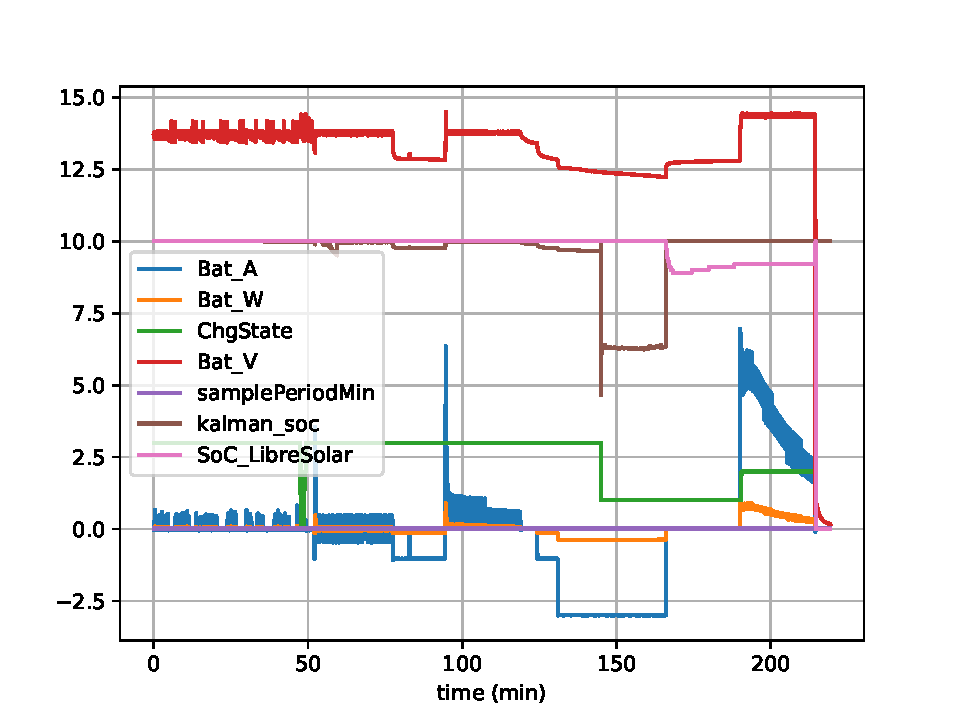
\includegraphics[width=16cm]{mppt-1210-hus-2021-05-28T20:10:00.000Z-2021-05-29T02:19:00.000Z-librevskalman-all.pdf}
\caption{\label{fig:librevskalman-mppt-1210-hus-all} SoC libre.solar algorithm vs kalman-soc on laboratory device mppt-1210-hus}
\end{figure}

In figure \ref{fig:librevskalman-mppt-hus} one can see that both algorithm have huge deviations, which might be due to a wrong capacity set in the charge controller. Still the kalman-soc algorithm follows well what one would expect by analyzing the charge state as well as the current and voltage. 

\begin{figure}
\centering	
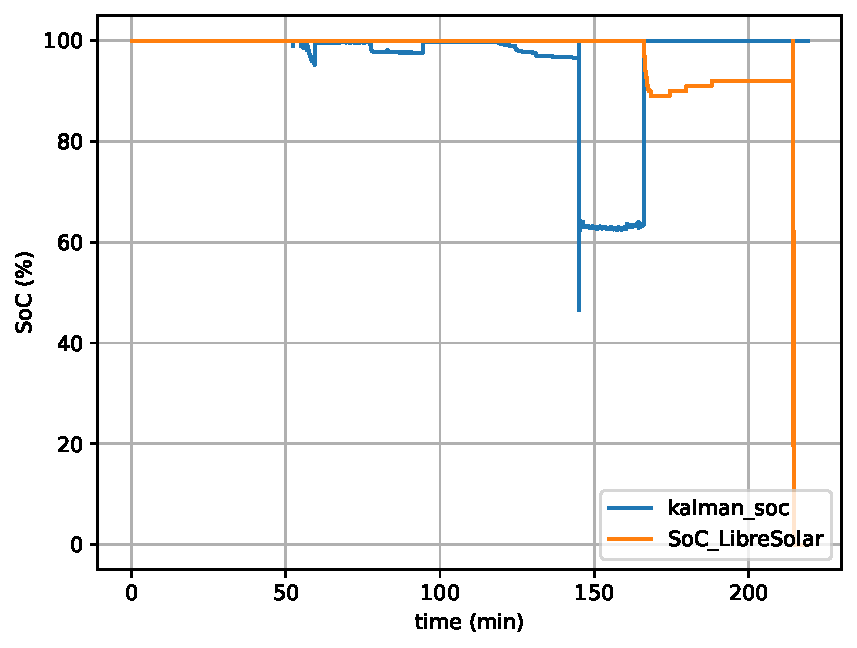
\includegraphics{mppt-1210-hus-2021-05-28T20:10:00.000Z-2021-05-29T02:19:00.000Z-librevskalman.pdf}
\caption{\label{fig:librevskalman-mppt-hus} SoC libre.solar algorithm vs kalman-soc on device mppt-1210-hus}
\end{figure}

\section{Dataset from EVLKpN of field test} 

The dataset introduced in figure \ref{fig:librevskalman-mppt-1210-hus-all} was produced by real world usage during 13 days in a household in Africa. 

\begin{figure}
\centering	
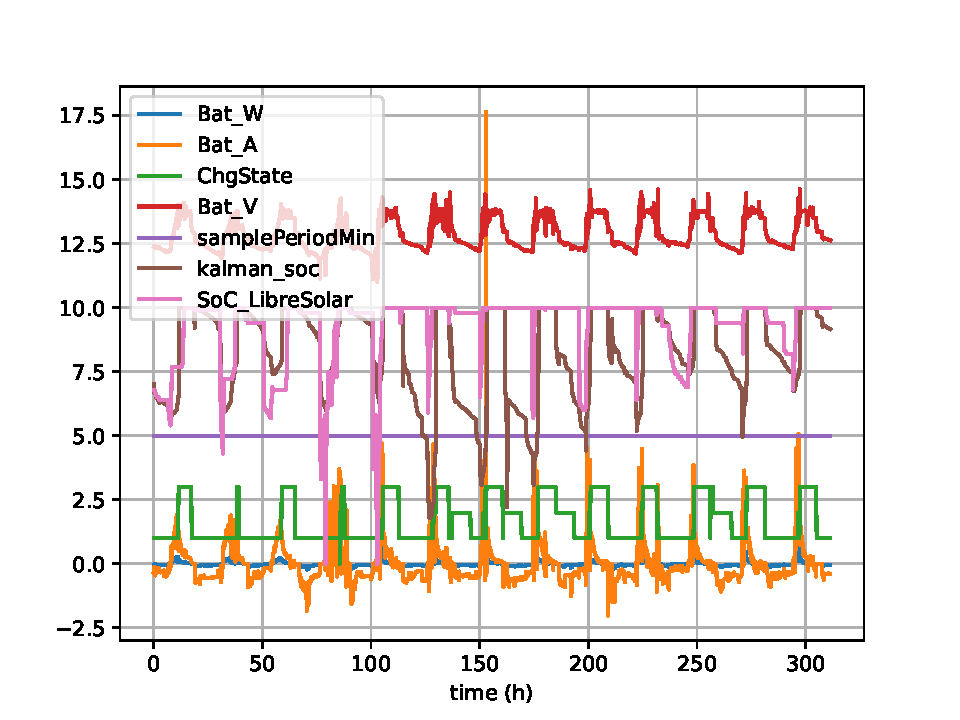
\includegraphics[width=16cm]{EVLKpN_20210817-20210830-librevskalman-all.pdf}
\caption{\label{fig:librevskalman-EVLKpN-all} SoC libre.solar algorithm vs kalman-soc on device EVLKpN in the field from from 2021/08/17 to 2021/08/30 }
\end{figure}


\begin{figure}
\centering	
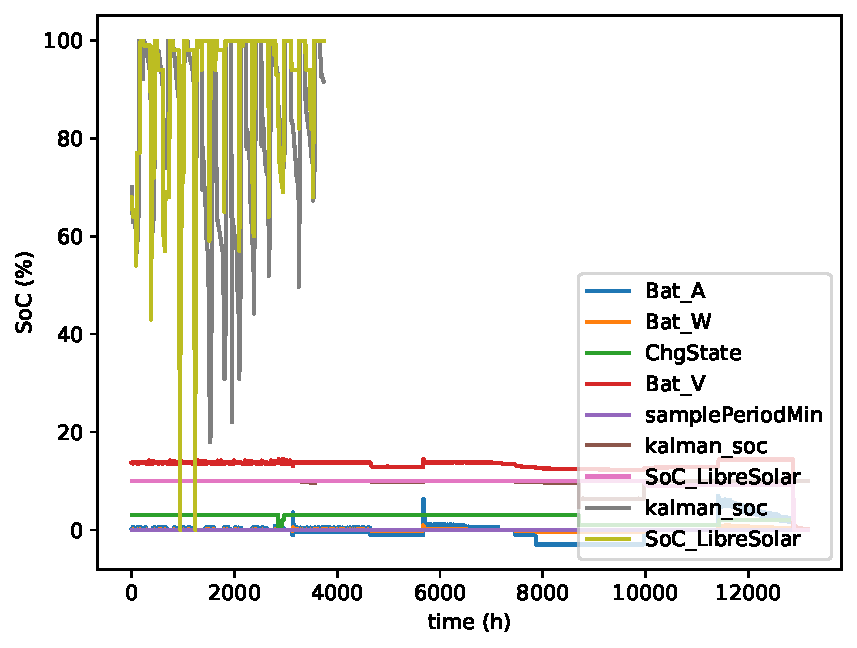
\includegraphics{EVLKpN_20210817-20210830-librevskalman.pdf}
\caption{\label{fig:librevskalman-EVLKpN} SoC libre.solar algorithm vs kalman-soc on device EVLKpN in the field from 2021/08/17 to 2021/08/30 }
\end{figure}



%\begin{pylabcode}
%#https://queirozf.com/entries/matplotlib-pylab-pyplot-etc-what-s-the-different-between-these
%#https://github.com/matplotlib/matplotlib/issues/10272hj
%import os 
%import pandas as pd
%currentWorkingDir =  os.getcwd()
%outputDataDir = currentWorkingDir + '/dep/kalman-soc/data/'
%dfProcessedSensorDataEnhanced = pd.read_csv(outputDataDir + 'EVLKpN_20210817-20210830_enhanced_processed_sensor_data.zip')  
%
%#Matplotlib
%dfProcessedSensorDataEnhanced.plot()
%plt.show()
%savefig('matplotoverview.pdf')
%
%#Plotly
%pd.options.plotting.backend = "plotly"
%fig = dfProcessedSensorDataEnhanced.plot()
%#fig.update_layout(title_text='<b> Overview  </b>', title_x=0.5)
%fig.show()
%fig.write_image("overview.pdf")
%\end{pylabcode}
	

%\begin{pylabcode}[plotsession]
%import os 
%import pandas as pd
%currentWorkingDir =  os.getcwd()
%outputDataDir = currentWorkingDir + '/dep/kalman-soc/data/'
%dfProcessedSensorDataEnhanced = pd.read_csv(outputDataDir + 'EVLKpN_20210817-20210830_enhanced_processed_sensor_data.zip')  
%
%x = dfProcessedSensorDataEnhanced.index
%yEKF = dfProcessedSensorDataEnhanced.kalman_soc
%ySoCLS = dfProcessedSensorDataEnhanced.SoC_LibreSolar
%# rc('text', usetex=True)
%# rc('font', **{'family':'serif', 'serif':['Times']})
%# rc('font', size=10.0)			
%# rc('legend', fontsize=10.0)
%#x = linspace(0, 3*pi)
%figure(figsize=(3.25,2))
%plot(x,yEKF,label='kalman_soc') 
%plot(x,ySoCLS,label='SoC_LibreSolar',linestyle='dashed')
%xlabel(r'time (min)')
%ylabel(r'SoC (\%)')
%#xticks(arange(0, 4*pi, pi), ('$0$',
%#'$\pi$', '$2\pi$', '$3\pi$'))
%#axis([0, 3*pi, -1, 1])
%legend(loc='lower right')
%savefig('librevskalman.pdf', bbox_inches='tight')
%\end{pylabcode}
%


\chapter{Conclusion}

The key to success for a good SoC is a good definition of both models and a good parametrization. % The implementation is independent of the use case and depends on the skills of the programmer, in his  hands lies the optimization of the  code.
In case no FPU is available on the micro-controller unit (MCU) fix point arithmetic might be an option. 
The Adaptive extend Kalman Filter (AEKF) is an option, where the parameters are determined online, but still AEKF needs to be initialized with parameters not necessary fitting all batteries of a given chemistry, because of different capacities or tolerances and specific designs. 
TODO It needs to be researched if it only affects the convergence time or if convergence is not reached at all? A further advantage of an adaptive filter is that the state of health (SOH) can be determined along the side. 
When simple observation and control-input models are used as in the okra kalman-soc algorithm, the parametrization might be much easier?
TODO to check if the initial parameters, in this case OCV in function of SoC data can be used generally or only on the batteries, the data has been generated with. \\

\textbf{Citations concerning the on/off-line parametrization} \\

"A sigma-point Kalman filter is further used to manage inaccuracies generated by the reduction process and experimental-related issues such as measurement error (noise) in the current and voltage sensors."


Offline parametrization: \\
'As a result, many experimental pretests investigating the
effects of the internal and external conditions of a battery on its parameters are required, since the
accuracy of state estimation depends on the quality of the information regarding battery parameter
changes'

'Therefore, some tests data must be available in 
advance to find the parameters of these models.'
\cite{hussein2011overview}  \\ \\ \\ \\

Gregory Plett says: \\
'Two possible approaches: \\

First, an algorithm might somehow adapt the parameter values of the model during operation to match presently observed current–voltage behaviors; but, this \textbf{must be done very carefully to avoid making the model unstable or physically nonmeaningful}. \\

Alternately, a set of models could be pre-computed at different feasible aging points and the model from this set that most closely predicts presently observed current–voltage dynamics could be selected from the set. This second approach guarantees stable and physically meaningful models since all models in the pre-computed set meet these criteria. We propose such an approach here.' 
---https://www.sciencedirect.com/science/article/abs/pii/S2352152X18301385?via%3Dihub
In order to have online first algo, the parametrization needs to be done online!. 



\subsection{Outlook} 

Promising articles and/or methods for online parameter estimation: \\ 

\textbf{online parameter estimation} from the ARX model {tran2017state}

\cite{wang2021augmented}
{xia2018online}
